%%%%%%%%%%%%%%%%%%%%%%%%%%%%%%%%%%%%%%%%%
% Beamer Presentation
% LaTeX Template
% Version 1.0 (10/11/12)
%
% This template has been downloaded from:
% http://www.LaTeXTemplates.com
%
% License:
% CC BY-NC-SA 3.0 (http://creativecommons.org/licenses/by-nc-sa/3.0/)
%
%%%%%%%%%%%%%%%%%%%%%%%%%%%%%%%%%%%%%%%%%

%----------------------------------------------------------------------------------------
%	PACKAGES AND THEMES
%----------------------------------------------------------------------------------------

\documentclass{beamer}

\mode<presentation> {
\usetheme{Madrid}
\setbeamertemplate{navigation symbols}{} % To remove the navigation symbols from the bottom of all slides uncomment this line
}	

\usepackage{graphicx} % Allows including images
\usepackage{booktabs} % Allows the use of \toprule, \midrule and \bottomrule in tables
\usepackage{color}
\usepackage{xcolor} %% http://www.ctan.org/pkg/xcolor
\usepackage{tikz}
\usepackage{gantt}
\newcommand\Fontvi{\fontsize{6}{7.2}\selectfont}
%----------------------------------------------------------------------------------------
%	TITLE PAGE
%----------------------------------------------------------------------------------------

\title[Corporate Governance and Performance]{The Relationship Between Corporate Governance and Company Performance \\~\\ \small {New factors, New models, New Approaches to Causality} } % The short title appears at the bottom of every slide, the full title is only on the title page

\author{Conor Reid} % Your name
\institute [UCD Smurfit School] % Your institution as it will appear on the bottom of every slide, may be shorthand to save space
{
UCD Michael Smurfit Graduate Business School \\
\medskip
\textit{conor.reid@ucdconnect.ie} % Your email address
}

\date{\today} % Date, can be changed to a custom date

\begin{document}

\begin{frame}
\titlepage % Print the title page as the first slide
\end{frame}

\begin{frame}
\frametitle{Overview} % Table of contents slide, comment this block out to remove it
\tableofcontents % Throughout your presentation, if you choose to use \section{} and \subsection{} commands, these will automatically be printed on this slide as an overview of your presentation
\end{frame}

%Put the logo on every page
\pgfdeclareimage[height=1.3cm]{logo}{images/logo.png}
\logo{\pgfuseimage{logo}\hspace*{0.5cm}}

%----------------------------------------------------------------------------------------
%	PRESENTATION SLIDES
%----------------------------------------------------------------------------------------
%------------------------------------------------
%------------------------------------------------
\section{Motivation and Previous Work}
\begin{frame}[t]
\frametitle{Motivation and Previous Work}
{Corporate governance models vary widely across firms, and there is much debate on the impact of these differing styles on company performance.
\begin{itemize}
\item[$\blacksquare$] How can these features be optimised for best performance?
\item[$\blacksquare$] What defines {\it best performance}? 
\end{itemize}
\vspace{1cm}
Moldovan and Mutu (M\&M, 2015) attempted to answer these questions. 
\begin{itemize}
\item[$\blacksquare$] Acquired data from Bloomberg financial system.
\item[$\blacksquare$] Worked to learn predictive models.
\item[$\blacksquare$] Proposed rules.
\end{itemize}
}
\end{frame}
{\small
\begin{frame}[t]
\frametitle{Motivation and Previous Work}
M\&M, 2015
\begin{itemize}
\item[$\checkmark$] Claimed numerous accurate correlations across multiple algorithms and measures.
\item [$\times$] Limited measures and features.
\item [$\times$] Unexplored algorithms and techniques.
\item [$\times$] Correlation $\neq$ Causation.
\end{itemize}
\vspace{0.5cm}
Other Work
\begin{itemize}
\item [$\blacksquare$] Pearl, Judea. (2009) discussed causality extensively.
\item[$\blacksquare$] King, G. et al. (2016) have proposed methodology causal inference.
\item [$\blacksquare$] Athey, S. (2017) have explored the gap between prediction \\and decision making.
\end{itemize}
\end{frame}
}
%------------------------------------------------ 
\section{Approach}
\begin{frame}[t]
\frametitle{Approach}
My Approach
\begin{enumerate}
\item Acquire data. \\~\\
\item Reproduce some of M\&M's results. \\~\\
\item Use alternative algorithms and techniques. \\~\\
\item Alternative features and measures of corporate governance and corporate success. \\~\\
\item Apply modern work in causation.
\end{enumerate}


%TODO: Flesh out
%\\~\\
%Replication and try to improve technically, then explore correlations to prove higher level meaning 
%\\~\\
%Try to use same data as M\&M and same algorithms to aid the above
%\\~\\

\end{frame}
%------------------------------------------------
\section {Academic Contribution}
\begin{frame}[t]
\frametitle{Academic Contribution}
{\it \small A deeper question concerns whether a given problem can be solved using only techniques for prediction, or whether statistical approaches to estimating the causal effect of an intervention are required. - Athey, S. (2017)}\\~\\
{Much research and development has gone into producing highly efficient prediction techniques, powered by the explosion of data. Causation is more difficult to prove.  }
%the availability of larger and more diverse datasets has made it possible for researchers to create better predictive models
%researchers have used the larger and more diverse datasets to.... 
\\~\\
{A significant contribution would be to examine and attempt to apply cutting edge research on proving causality to this domain.}

%{This project will examine and attempt to apply cutting edge research on proving causality to this domain. This would be a significant contribution to the field.    }
%using modern work in causality 
%is intended to extend mm by applying modern findings on / in causality to the bloomberg dataset  
\end{frame}
%------------------------------------------------
\section {Practical Application}
\begin{frame}[t]
\frametitle{Practical Application}
\begin{itemize}
\item[$\blacksquare$] Data based decisions need to consider causality, not just correlation.
\\~\\
\item[$\blacksquare$] Domain specific practicality, propose best practice for corporate governance.
\end{itemize}
\begin{figure}[h]
\centering 
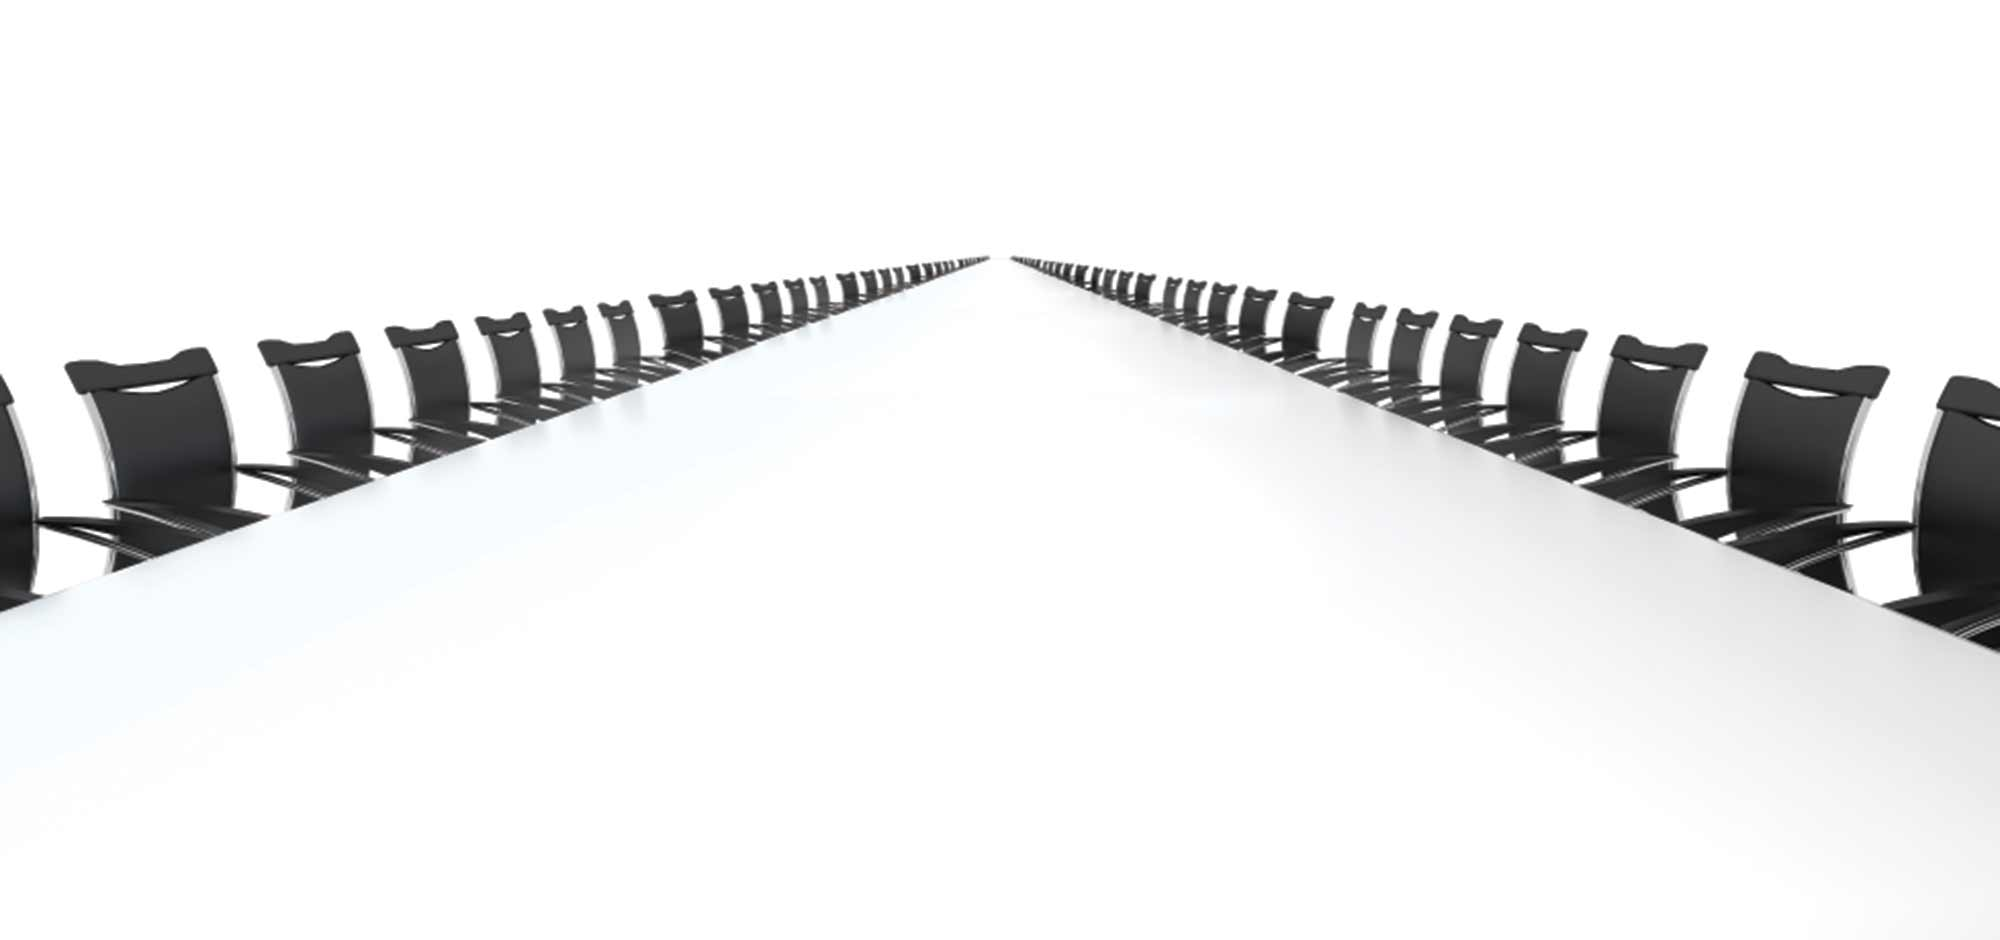
\includegraphics[scale=0.1]{images/boardroom.jpg}
\end {figure}

\end{frame}
%------------------------------------------------
\section {Data Requirements}
\begin{frame}[t]
\frametitle{The Data}
%make two slides out of this
%remove equations 

Three stock indexes considered: \\

\begin{itemize}
  \item[]
  S\&P500 (SPX) %moodys

  \item[]
  STOXX Europe 600 (SXXP)
  \hspace{1.3cm}    $\smash{\left.\rule{0pt}{.5\dimexpr3\baselineskip+\itemsep+6\parskip}\right\}
      \text{M\&M: 1400, 52 }}$

  \item[]
  STOXX Eastern Europe 300 (EEBP)
\end{itemize}
\vspace{0.6cm}
Explanatory Variables: \\~\\
%{\small 
%$Tobin's \; Q = \frac{(\; Market \; Cap \; + \; Total \; Liabilities \; + \; Preferred \; Equity \; + \;Minority \; Interest \;)}{Total \; Assets}$}
 %\\~\\
Tobin's Q $\propto  Market \; Cap, Total \; Liabilities, Preferred \; Equity \; etc. $
 \\~\\
%{\small
%$Altman \; Z \; Score = 1.2  \; (\frac{Working \; Capital}{Tangible \; Assets}) + 1.4  \; (\frac{Retained \; Earnings}{Tangible \; Assets})
%+ 3.3 \; (\frac{EBIT}{Tangible \;Assets})
%+ 0.6 \; (\frac{Market \; Value \; of \; Equity}{Total \; Liabilities})
%+ \frac{Sales}{TangibleAssets}$}
Altman Z Score $\propto  Working \; Capital, Tangible \; Assets, Market \; Value \;  etc. $


\end{frame}
\begin{frame}[t]
\frametitle{The Data}
\begin{columns}
\column{0.55\textwidth}
Sourcing the Data: \\
\begin{enumerate}
\item Directly from the authors
	\begin{itemize}
	\item[\checkmark]{Replicate their study.}	
	%look up Expedites
	\item[\checkmark]{Expedites the project.}
	\item [] This request is with M\&M. 
	\end{itemize}
\vspace{1cm}	
\item Extract it myself
	\begin{itemize}
	\item[\checkmark]{More autonomy.}	
	\item[\checkmark]{Gain experience with Bloomberg.}
	\item[$\times$]{Time commitment.}
	\end{itemize}
\end{enumerate}

\column{0.45\textwidth}
%\vspace{6cm}
\begin{figure}[h]
\centering
\includegraphics[scale=0.4]{images/Bloomberg-Terminal.jpg}
\end{figure}
\end{columns}





\end{frame}

%------------------------------------------------
\section {Measuring Success}
\begin{frame}[t]
\frametitle{Measuring Success}
Project Goals
\begin{itemize}
\item[$\circlearrowright$] Consider auxiliary features beyond the current dataset. \\~\\
\item[$\blacksquare$] Reproduce some of M\&M's findings and seek to improve on results. \\~\\
\item[$\blacksquare$] Carry out new techniques. \\~\\
\item[$\sim$] Investigate and apply modern work on causality.
\end{itemize}
\end{frame}
%------------------------------------------------
\section {Project Timeline}


\iffalse
\begin{frame}[t]
\frametitle{Project Timeline - WIP}
TODO: Flesh out - Figure out a timeline tool
\\~\\
{\small 
Consider deadlines for submission to conferences / journals
\\~\\
Submission of papers January 15th 2018 (for same conference as M\&M) Try to get as much done this coming summer re. replicating / technical work. Leave time to explore research on causation?
}
\begin{tikzpicture}[]
%draw horizontal line
\draw (0,0) -- (15/1.7,0);
%draw vertical lines
\foreach \x in {0, 8, 15, 22, 29, 36, 41}{
   \draw (\x/1.7,3pt) -- (\x/1.7,-3pt);
}
%draw nodes
\draw (0,0) node[below=3pt] { 1 } node[above=3pt] { Jan 13 2014  };
\draw (8/1.7,0) node[below=3pt] { 2 } node[above=3pt] { Jan 20 2014  };
\end{tikzpicture}
\\~\\
\begin{tikzpicture}[]
%draw horizontal line
\draw (0,0) -- (15/1.7,0);
%draw vertical lines
\foreach \x in {0, 8, 15, 22, 29, 36, 41}{
   \draw (\x/1.7,3pt) -- (\x/1.7,-3pt);
}
%draw nodes
\draw (0,0) node[below=3pt] { 1 } node[above=3pt] { Jan 13 2014  };
\draw (8/1.7,0) node[below=3pt] { 2 } node[above=3pt] { Jan 20 2014  };
\end{tikzpicture}

\end{frame}
\fi
%------------------------------------------------
\begin{frame}[t]
\frametitle{Project Timeline}
  \hspace{0.25cm}
  %\begin{center}
    \scalebox{0.6}{    
	%\begin{gantt}{12}{20}
	\begin{gantt}{9}{12}
	\begin{ganttitle}
      	\titleelement{\large 2017}{12}
	%\titleelement{2018}{8}
    	\end{ganttitle}
    	\begin{ganttitle}
	\titleelement{\large Jan}{1}
	\titleelement{\large Feb}{1}
	\titleelement{\large Mar}{1}
	\titleelement{\large Apr}{1}
	\titleelement{\large May}{1}
	\titleelement{\large Jun}{1}
	\titleelement{\large Jul}{1}
	\titleelement{\large Aug}{1}
	\titleelement{\large Sept}{1}
	\titleelement{\large Oct}{1}
	\titleelement{\large Nov}{1}
	\titleelement{\large Dec}{1}
	%\titleelement{Jan}{1}
	%\titleelement{Feb}{1}
	%\titleelement{Mar}{1}
	%\titleelement{Apr}{1}
	%\titleelement{May}{1}
	%\titleelement{Jun}{1}
	%\titleelement{Jul}{1}
	%\titleelement{Aug}{1}
	\end{ganttitle}
	 \ganttbar{Project Initialisation}{0}{2}
	  \ganttbar{Reading}{1}{11}
	 \ganttbar{Proposal presentation}{2}{1}
	 \ganttbar{Acquire Data}{2}{4}
	 \ganttbar{Replicate M\&M}{5}{3}
	 \ganttbar{Apply Causation Work}{8}{4}
	 \ganttbar{Write Conference Paper}{10}{2}
	 %\ganttbar{\small Submit Paper to Conference}{12}{1}
	 %\ganttbar{\small Contingency}{13}{6}
	 %\ganttbar{\small Project Submission}{19}{1}
     \end{gantt}
        }
    %\end{center}
    
    
    %  \begin{center}
    \scalebox{0.6}{    
	\begin{gantt}{5}{8}
	\begin{ganttitle}
      	\titleelement{\large 2018}{8}
    	\end{ganttitle}
    	\begin{ganttitle}
	\titleelement{\large Jan}{1}
	\titleelement{\large Feb}{1}
	\titleelement{\large Mar}{1}
	\titleelement{\large Apr}{1}
	\titleelement{\large May}{1}
	\titleelement{\large Jun}{1}
	\titleelement{\large Jul}{1}
	\titleelement{\large Aug}{1}
	\end{ganttitle}
	 \ganttbar{Publish to Conference}{0}{1}
	 \ganttbar{Contingency}{1}{6}
	 \ganttbar{Project Submission to UCD}{7}{1}
     \end{gantt}
        }
    %\end{center}
    
\end{frame}
\begin{frame}
\Huge{\centerline{Thank You.}}
\end{frame}






%------------------------------------------------
%------------------------------------------------

%----------------------------------------------------------------------------------------
%	COMMENTS
%----------------------------------------------------------------------------------------
\iffalse
\begin{frame}
{Test}
\end{frame}


\begin{frame}
\frametitle{Paragraphs of Text}
Sed iaculis dapibus gravida. Morbi sed tortor erat, nec interdum arcu. Sed id lorem lectus. Quisque viverra augue id sem ornare non aliquam nibh tristique. Aenean in ligula nisl. Nulla sed tellus ipsum. Donec vestibulum ligula non lorem vulputate fermentum accumsan neque mollis.\\~\\

Sed diam enim, sagittis nec condimentum sit amet, ullamcorper sit amet libero. Aliquam vel dui orci, a porta odio. Nullam id suscipit ipsum. Aenean lobortis commodo sem, ut commodo leo gravida vitae. Pellentesque vehicula ante iaculis arcu pretium rutrum eget sit amet purus. Integer ornare nulla quis neque ultrices lobortis. Vestibulum ultrices tincidunt libero, quis commodo erat ullamcorper id.
\end{frame}

%------------------------------------------------

\begin{frame}
\frametitle{Bullet Points}
\begin{itemize}
\item Lorem ipsum dolor sit amet, consectetur adipiscing elit
\item Aliquam blandit faucibus nisi, sit amet dapibus enim tempus eu
\item Nulla commodo, erat quis gravida posuere, elit lacus lobortis est, quis porttitor odio mauris at libero
\item Nam cursus est eget velit posuere pellentesque
\item Vestibulum faucibus velit a augue condimentum quis convallis nulla gravida
\end{itemize}
\end{frame}

%------------------------------------------------

\begin{frame}
\frametitle{Multiple Columns}
\begin{columns}[c] % The "c" option specifies centered vertical alignment while the "t" option is used for top vertical alignment

\column{.45\textwidth} % Left column and width
\textbf{Heading}
\begin{enumerate}
\item Statement
\item Explanation
\item Example
\end{enumerate}

\column{.5\textwidth} % Right column and width
Lorem ipsum dolor sit amet, consectetur adipiscing elit. Integer lectus nisl, ultricies in feugiat rutrum, porttitor sit amet augue. Aliquam ut tortor mauris. Sed volutpat ante purus, quis accumsan dolor.

\end{columns}
\end{frame}

%------------------------------------------------
\section{Second Section}
%------------------------------------------------

\begin{frame}
\frametitle{Table}
\begin{table}
\begin{tabular}{l l l}
\toprule
\textbf{Treatments} & \textbf{Response 1} & \textbf{Response 2}\\
\midrule
Treatment 1 & 0.0003262 & 0.562 \\
Treatment 2 & 0.0015681 & 0.910 \\
Treatment 3 & 0.0009271 & 0.296 \\
\bottomrule
\end{tabular}
\caption{Table caption}
\end{table}
\end{frame}

%------------------------------------------------

\begin{frame}
\frametitle{Theorem}
\begin{theorem}[Mass--energy equivalence]
$E = mc^2$
\end{theorem}
\end{frame}



%------------------------------------------------

\begin{frame}
\Huge{\centerline{The End}}
\end{frame}


%----------------------------------------------------------------------------------------
\fi
\end{document}